%%
% Copyright (c) 2017 - 2020, Pascal Wagler;
% Copyright (c) 2014 - 2020, John MacFarlane
%
% All rights reserved.
%
% Redistribution and use in source and binary forms, with or without
% modification, are permitted provided that the following conditions
% are met:
%
% - Redistributions of source code must retain the above copyright
% notice, this list of conditions and the following disclaimer.
%
% - Redistributions in binary form must reproduce the above copyright
% notice, this list of conditions and the following disclaimer in the
% documentation and/or other materials provided with the distribution.
%
% - Neither the name of John MacFarlane nor the names of other
% contributors may be used to endorse or promote products derived
% from this software without specific prior written permission.
%
% THIS SOFTWARE IS PROVIDED BY THE COPYRIGHT HOLDERS AND CONTRIBUTORS
% "AS IS" AND ANY EXPRESS OR IMPLIED WARRANTIES, INCLUDING, BUT NOT
% LIMITED TO, THE IMPLIED WARRANTIES OF MERCHANTABILITY AND FITNESS
% FOR A PARTICULAR PURPOSE ARE DISCLAIMED. IN NO EVENT SHALL THE
% COPYRIGHT OWNER OR CONTRIBUTORS BE LIABLE FOR ANY DIRECT, INDIRECT,
% INCIDENTAL, SPECIAL, EXEMPLARY, OR CONSEQUENTIAL DAMAGES (INCLUDING,
% BUT NOT LIMITED TO, PROCUREMENT OF SUBSTITUTE GOODS OR SERVICES;
% LOSS OF USE, DATA, OR PROFITS; OR BUSINESS INTERRUPTION) HOWEVER
% CAUSED AND ON ANY THEORY OF LIABILITY, WHETHER IN CONTRACT, STRICT
% LIABILITY, OR TORT (INCLUDING NEGLIGENCE OR OTHERWISE) ARISING IN
% ANY WAY OUT OF THE USE OF THIS SOFTWARE, EVEN IF ADVISED OF THE
% POSSIBILITY OF SUCH DAMAGE.
%%

%%
% This is the Eisvogel pandoc LaTeX template.
%
% For usage information and examples visit the official GitHub page:
% https://github.com/Wandmalfarbe/pandoc-latex-template
%%


% @modified: Chuwen <chuwzhang@gmail.com>
% Options for packages loaded elsewhere
\PassOptionsToPackage{unicode}{hyperref}
\PassOptionsToPackage{hyphens}{url}
\PassOptionsToPackage{dvipsnames,svgnames*,x11names*,table}{xcolor}
%
\documentclass[
  a4paper,
  ,tablecaptionabove
]{scrartcl}
\usepackage{lmodern}
\usepackage{setspace}
\setstretch{1.2}
\usepackage{amssymb,amsmath}
\numberwithin{equation}{section}
\usepackage{ifxetex,ifluatex}
\usepackage{unicode-math}
\defaultfontfeatures{Scale=MatchLowercase}
\defaultfontfeatures[\rmfamily]{Ligatures=TeX,Scale=1}

% Use upquote if available, for straight quotes in verbatim environments
\IfFileExists{upquote.sty}{\usepackage{upquote}}{}
\IfFileExists{microtype.sty}{% use microtype if available
  \usepackage[]{microtype}
  \UseMicrotypeSet[protrusion]{basicmath} % disable protrusion for tt fonts
}{}
\makeatletter
\@ifundefined{KOMAClassName}{% if non-KOMA class
  \IfFileExists{parskip.sty}{%
    \usepackage{parskip}
  }{% else
    \setlength{\parindent}{0pt}
    \setlength{\parskip}{6pt plus 2pt minus 1pt}}
}{% if KOMA class
  \KOMAoptions{parskip=half}}
\makeatother
\usepackage{xcolor}
\definecolor{default-linkcolor}{HTML}{A50000}
\definecolor{default-filecolor}{HTML}{A50000}
\definecolor{default-citecolor}{HTML}{4077C0}
\definecolor{default-urlcolor}{HTML}{4077C0}
\IfFileExists{xurl.sty}{\usepackage{xurl}}{} % add URL line breaks if available
\IfFileExists{bookmark.sty}{\usepackage{bookmark}}{\usepackage{hyperref}}
\hypersetup{
  pdfauthor={Chuwen},
  hidelinks,
  breaklinks=true,
  pdfcreator={LaTeX via pandoc with the Eisvogel template}}
\urlstyle{same} % disable monospaced font for URLs
\usepackage[margin=2.5cm,includehead=true,includefoot=true,centering,]{geometry}
% add backlinks to footnote references, cf. https://tex.stackexchange.com/questions/302266/make-footnote-clickable-both-ways
\usepackage{footnotebackref}
\usepackage{graphicx,grffile}
\makeatletter
\def\maxwidth{\ifdim\Gin@nat@width>\linewidth\linewidth\else\Gin@nat@width\fi}
\def\maxheight{\ifdim\Gin@nat@height>\textheight\textheight\else\Gin@nat@height\fi}
\makeatother
% Scale images if necessary, so that they will not overflow the page
% margins by default, and it is still possible to overwrite the defaults
% using explicit options in \includegraphics[width, height, ...]{}
\setkeys{Gin}{width=\maxwidth,height=\maxheight,keepaspectratio}
\setlength{\emergencystretch}{3em}  % prevent overfull lines
\providecommand{\tightlist}{%
  \setlength{\itemsep}{0pt}\setlength{\parskip}{0pt}}
\setcounter{secnumdepth}{3}

% Make use of float-package and set default placement for figures to H.
% The option H means 'PUT IT HERE' (as  opposed to the standard h option which means 'You may put it here if you like').
\usepackage{float}
\floatplacement{figure}{H}
\usepackage{amsthm}
\usepackage[ruled,vlined]{algorithm2e}
\newtheorem{theorem}{Theorem}[section]
\newtheorem{corollary}{Corollary}[theorem]
\newtheorem{lemma}[theorem]{Lemma}
\newtheorem{prop}{Proposition}

%
% language specification
%
% If no language is specified, use English as the default main document language.
%
\usepackage{polyglossia}
\setmainlanguage[]{english}

\usepackage[UTF8, heading=true]{ctex}
\usepackage{booktabs}
\definecolor{tufeijilk}{RGB}{68,87,151}
\hypersetup{colorlinks=true,linkcolor=tufeijilk,urlcolor=cyan}
\newlength{\cslhangindent}
\setlength{\cslhangindent}{1.5em}
\newenvironment{cslreferences}%
{}%
{\par}

%
% break urls
%
\PassOptionsToPackage{hyphens}{url}

%
% When using babel or polyglossia with biblatex, loading csquotes is recommended
% to ensure that quoted texts are typeset according to the rules of your main language.
%
\usepackage{csquotes}

%
% captions
%
\definecolor{caption-color}{HTML}{777777}
\usepackage[font={stretch=1.2}, textfont={color=caption-color}, position=top, skip=4mm, labelfont=bf, singlelinecheck=false, justification=raggedright]{caption}
\setcapindent{0em}

%
% blockquote
%
\definecolor{blockquote-border}{RGB}{221,221,221}
\definecolor{blockquote-text}{RGB}{119,119,119}
\usepackage{mdframed}
\newmdenv[rightline=false,bottomline=false,topline=false,linewidth=3pt,linecolor=blockquote-border,skipabove=\parskip]{customblockquote}
\renewenvironment{quote}{\begin{customblockquote}\list{}{\rightmargin=0em\leftmargin=0em}%
    \item\relax\color{blockquote-text}\ignorespaces}{\unskip\unskip\endlist\end{customblockquote}}

%
% heading color
%
\definecolor{heading-color}{RGB}{40,40,40}
\addtokomafont{section}{\color{heading-color}}
% When using the classes report, scrreprt, book,
% scrbook or memoir, uncomment the following line.
%\addtokomafont{chapter}{\color{heading-color}}

%
% variables for title and author
%
\usepackage{titling}

%
% tables
%
\usepackage{array}
\usepackage{multirow}
\usepackage{longtable}
%
% remove paragraph indention
%
\setlength{\parindent}{0pt}
\setlength{\parskip}{6pt plus 2pt minus 1pt}
\setlength{\emergencystretch}{3em}  % prevent overfull lines

%
%
% Listings
%
%


%
% header and footer
%
\usepackage{fancyhdr}

\fancypagestyle{eisvogel-header-footer}{
  \fancyhead{}
  \fancyfoot{}
  \lhead[\today]{}
  \chead[]{}
  \rhead[]{\today}
  \lfoot[\thepage]{Chuwen}
  \cfoot[]{}
  \rfoot[Chuwen]{\thepage}
  \renewcommand{\headrulewidth}{0.4pt}
  \renewcommand{\footrulewidth}{0.4pt}
}
\pagestyle{eisvogel-header-footer}


\usepackage{natbib}
\bibpunct[, ]{(}{)}{,}{a}{}{,}%
\def\bibfont{\small}%
\def\bibsep{\smallskipamount}%
\def\bibhang{24pt}%
\def\newblock{\ }%
\def\BIBand{and}%

\usepackage{svg}
\svgpath{fig}

%
% variables for title and author
%
\author{Chuwen}
\date{\today}


\title{}


%%
%% end added
%%

\begin{document}

{
\setcounter{tocdepth}{3}
\tableofcontents
}
\hypertarget{lagrangian-relaxation}{%
  \section{Lagrangian relaxation}\label{lagrangian-relaxation}}

Consider the following newsvendor-like problem
\begin{equation}\label{eq:primal}
  \begin{aligned}
                  & \min f(\delta, \epsilon)                                                                       \\
    \mathbf{s.t.} &                                                                                                \\
                  & y + \delta - \epsilon = b                                                                      \\
                  & y \in \Omega_y \subseteq \mathbb{R}^n, \delta \in \mathbb{R}^n_+ , \epsilon \in \mathbb{R}^n_+
  \end{aligned}
\end{equation}

where \(f\) is a convex function of \(\delta, \epsilon\). The
right-hand-side on the binding constraints is in the positive orthant:
\(b \in \mathbb R_+^n\).  In the basic
settings, let \(y\) be the ordering quantity quantities in a multi-item multi-period
newsvendor problem, one minimizes the total expected cost:

\[\min_{y \in \mathbb R_+} \mathbf E\left(h\cdot e^\mathsf{T} \max\{y - b,  0\} + p \cdot e^\mathsf{T} \max\{b - y,  0\}\right)\]

It is easy to verify the equivalence of the deterministic version, i.e., without the expectation operator, to the problem above. This problem widely appears in applications of
device maintenance, inventory management, crew scheduling and so on.

Let \(\lambda\in\mathbb{R}^n\) be the Lagrangian multiplier, the dual
function is:

\begin{equation}\label{eq:dual}
  \begin{aligned}
    \phi(\lambda) = & \min_{\delta, \epsilon} f(\delta, \epsilon) + \lambda^\mathsf{T}\delta - \lambda^\mathsf{T} \epsilon+ \min_y \lambda^\mathsf{T} y - \lambda^\mathsf{T} b \\
    \mathbf{s.t.}   &                                                                                                                                                          \\
                    & y \in \Omega_y                                                                                                                                           \\
                    & \delta \in \mathbb{R}^n_+ , \epsilon \in \mathbb{R}^n_+
  \end{aligned}
\end{equation}

We assume the resulting two subproblems for \(\delta, \epsilon\) and
\(y\) are easy. Denote $f^\star, \phi^\star$ be the optimal objective for primal and dual problem, respectively.

\hypertarget{affine-case}{%
  \subsection{Affine case}\label{affine-case}}

\textbf{The case for repair problem}

Let \(f=p^\mathsf{T}\delta + h^\mathsf{T} \epsilon\), we have

\[\phi(\lambda) = \min_{\delta, \epsilon} (p+ \lambda)^\mathsf{T}\delta + (h - \lambda)^\mathsf{T} \epsilon+ \min_y \lambda^\mathsf{T} y - \lambda^\mathsf{T} b\]

Then \(\phi\) is unbounded unless \(\lambda \in \Lambda\) where
\(\Lambda = \{\lambda: \lambda \in [-p, h]\}\), in which case

\[\phi(\lambda) = \min_{y\in \Omega_y} \lambda^\mathsf{T} y - \lambda^\mathsf{T} b,\; \lambda\in \Lambda\]

and \(\delta^\star(\lambda), \epsilon^\star(\lambda)= 0\) are corresponding optimizers
for any \(\lambda \in \Lambda\)

\hypertarget{conditions-for-strong-duality}{%
  \subsection{Conditions for strong
    duality}\label{conditions-for-strong-duality}}

It's well known that strong duality does not hold in general. We review
some of the cases here. The Lagrangian duality theory can be found in
any standard text.

\begin{theorem}
  if \(\Omega_y\) is convex then the strong duality holds ...,
  i.e.~\(\phi^\star = f^\star\)
\end{theorem}

add justifications here (slater, ...)

A more interesting result is devoted to mixed integer problems.
We know Lagrangian relaxation produces a bound up to
linear relaxation of a problem with the "easy" constraints
and the convex hull of relaxed constraints.

\textbf{(Review Here)}.

\begin{lemma}
  if \(\Omega_y = \{y \in \mathbb R^n: y \in \Omega, y\in \mathbb Z^n\}\).
  Then we have the following relation for dual function,
  \[ \phi^\star = \min_{\delta, \epsilon} f(\delta, \epsilon)\quad \textbf{ s.t. }  y + \delta - \epsilon = b,\; y \in \textrm{conv}(\Omega_y)\]
\end{lemma}

This immediately allows us to have strong duality by definition of perfect formulation,
in which case the linear relaxation solves the original problem.

\begin{corollary}\label{strong-ip}
  We conclude the strong duality holds since
  \(Y = \{(y, \delta, \epsilon): y + \delta - \epsilon = b,\; y \in \textsf{conv}(\Omega_y)\}\)
  is already \emph{a perfect formulation} in the sense that
  \(Y = \textsf{conv}(Y)\)
\end{corollary}

\textbf{show this or add more conditions to
  justify}


\hypertarget{subgradient-method}{%
  \section{Subgradient method}\label{subgradient-method}}

To solve the reduced problem for $\lambda$, we consider a class of subgradient
methods:

\begin{equation}\lambda_{k+1} = \mathbf{P}(\lambda_{k} + s_{k}d_{k})\end{equation}

where \(\mathbf P\) is the projection onto dual space \(\Lambda\).
\(d_k\) is the update direction for current iteration and \(s_{k}\) is
the step size using target-based rule:

\begin{equation}\label{eq:step_size}
  s_{k} = \gamma_k\frac{\phi^\star - \phi(\lambda_k)}{||d_{k}||^2}
\end{equation}

Note the direction \(d_k\) computed by

\begin{equation}\label{eq:direction}
  d_k = \bar y_k - b
\end{equation}

where \(\bar y_k\) is the convex combination of previous iterations
\(\{y_i\}_{i=1,...k}\) and each \(y_i\) solves
\(\phi_i = \phi(\lambda_i)\):

\begin{equation}\bar y_k = \sum^i_k \alpha^i_k y_i,\quad  \sum^i_k \alpha^i_k = 1, \alpha^i_k \ge 0\end{equation}

Alternatively, one can express the convexity in a recursive manner:

\begin{equation}\bar y_k = (1-\alpha_k)\cdot\bar y_{k-1} + \alpha_k \cdot y_k \end{equation}

For we simplicity take \(g_k= y_k - b\), then \(g_k\) is a subgradient
of \(\phi\) at \(\lambda_k\):

\begin{equation}g_k \in \partial \phi_k\end{equation}

The direction can be rewritten as the combination of the subgradient and
previous directions:

\begin{equation}\label{eq:direction_recursive}
  d_k = (1-\alpha_k) \cdot d_{k-1} + \alpha_k\cdot g_k
\end{equation}


The dual subgradient algorithm can be summarized as follows.
\(\varepsilon,\varepsilon_s\) are the tolerance parameter for objective gap and stepsize, respectively.
\(\varepsilon > 0 ,\varepsilon_s > 0\).

\begin{algorithm}[H]
  \SetAlgoLined
  Initialization. \(\alpha_0 = 1, \lambda_0 = e, \gamma_0 = 1\)  \\
  \While{\(\bar z_k - \phi_k \ge \varepsilon\) \textbf{and} \(s_k \ge \varepsilon_s\)}
  {
    Let current iteration be \(k\)\\
    Update the multipliers by
    \[\lambda_{k} = \mathbf{P}(\lambda_{k-1} + s_{k-1}d_{k-1})\]

    Solve dual problem \(\phi_k\) by \eqref{eq:dual}
    and compute subgradient \(g_k\) respectively.

    Compute \(\gamma_k, \alpha_k\) properly.

    Compute current direction by \eqref{eq:direction} or \eqref{eq:direction_recursive}

    Update \(\epsilon_k,\delta_k ,\bar \epsilon_k ,\bar \delta_k, z_k, \bar z_k \)
    by the \underline{Recovery Algorithm} \ref{alg:recovery}

    Stepsize is updated by \eqref{eq:step_size}
  }
  \caption{The Subgradient Algorithm}
\end{algorithm}

It is obvious to see the solutions during dual optimization
\((y, \epsilon, \delta) = (y_k, 0, 0)\) are feasible if and only if we
can find \(y_k = d\), which in general will not hold. This motivates the following
algorithm based on linear programming theory.

\begin{algorithm}[H]\label{alg:recovery}
  \SetAlgoLined
  \begin{equation}\label{eq:recovery}
    \begin{aligned}
       & \epsilon_k = \max\{y_k - b, 0\}           \\
       & \delta_k = \max\{b - y_k, 0\}             \\
       & \bar \epsilon_k = \max\{\bar y_k - b, 0\} \\
       & \bar \delta_k = \max\{b - \bar y_k, 0\}
    \end{aligned}\end{equation}
  \caption{Recovery Algorithm}
\end{algorithm}

To simplify our presentation, let
\(z\) be a function of \(y\) such that \(z_k = z(y_k) = f(\delta_k, \epsilon_k)\), then \(z\) is
also convex in \(y\) since both function \(f\) and \(\max\{\cdot, 0\}\)
are convex. It's also worth to notice that \(\bar \epsilon_k\) should
not be calculated as running averages:
\(\bar \epsilon_k \neq \sum^i_k \alpha^i_k \epsilon_i\). For such an
``averaged'' solution, we let
\(\bar z_k = z(\bar y_k)\). We later find the recovery algorithm achieves
at the optimal objective.


\hypertarget{convergence}{%
  \section{Convergence}\label{convergence}}


We first review several features for the subgradient method regarding
parameters \(\gamma_k, \alpha_k\) and search direction \(d_k\) produced from convex combinations.

The target based rule are well-known as the Polyak rule \cite{polyak_general_1967}.
The idea of using previous searching directions is introduced to accelerate the subgradient method and provide a better stopping criterion,
see \cite{camerini1975improving}, \cite{brannlund1995generalized}, \cite{barahona_volume_2000}.
\cite{brannlund1995generalized} showed that with convex combinations the optimal choice of stepsize is
equivalent to the Camerini-Fratta-Maffioli modification, it also provides an analysis on its linear convergence rate.

From the primal perspective, our method is close to \emph{primal
  averaging method}. \cite{nedic_approximate_2009}
gives a line of analysis on convergence and quality of the primal
approximation by averaging over all previous solutions with a constant
stepsize. They use a simple averaging scheme that can be rephrased into a
recursive equation with \(\alpha_k = 1/k\) such that:

\[\bar y_k = \frac{k-1}{k}\cdot\bar y_{k-1} + \frac{1}{k} \cdot y_k\]

then it gives lower and upper bounds for the averaged solution
that involve the primal violation, norm of the subgradient, etc. Furthermore, they only analyze the case for constant
stepsize \(s_k = s, s\ge 0\) and the search direction defined solely by
the subgradient. We refer to \cite{kiwiel_lagrangian_2007} for target based
stepsizes. The volume algorithm proposed by \cite{barahona_volume_2000} is close to the
case mentioned in \cite{brannlund1995generalized} in a dual
viewpoint while adopting \(\hat \lambda_{k}\) instead of \(\lambda_k\) from the best dual bound
\(\hat \phi_k = \max_{i=1, ..., k} \phi(\lambda_i)\):

\[\lambda_{k+1} = \mathbf{P}(\hat\lambda_{k} + s_{k}d_{k})\]

\emph{There is no existing proof of convergence} for the volume
algorithm, and our experiments show that the algorithm converges to
non-optimal solutions occasionally.

\textbf{(Remark / Difference for our method)}

Since the solution is strictly feasible by implementation of the
recovery algorithm \ref{eq:recovery}, i.e., there is no need to bound for feasibility gap
as has been done in most of literature covering the \textbf{primal
  recovery}. Instead, we have analyze the quality of the heuristic, i.e.:

\[
  |\bar z_k - \phi_k| \textrm { or } |\bar z_k - z^\star|
\]

We found its convergence is closely related to strong duality of the problem. Accounting for performance,
we suggest several specific choices of parameters regarding the subgradient method \((\gamma, \alpha, d)\).


\hypertarget{analysis-outline}{%
  \subsection{Analysis outline}\label{analysis-outline}}

\begin{itemize}
  \tightlist
  \item
        we've showed \hyperlink{conditions for strong-duality}{zero duality gap}
        \(\phi^\star = f^\star= z^\star\)
  \item
        we show \(\lambda_k\) converges to \(\lambda^\star \in \Lambda^\star\)
        for our choices of \(\gamma_k, \alpha_k\)
  \item
        we show primal solution \(\bar z_k\) converges to \(z^\star\)
\end{itemize}

\begin{lemma}\(\epsilon\)-subgradient.
  \begin{equation}\label{eq:subgrad}
    \begin{aligned}
      g_{k}^\mathsf{T}(\lambda_{k}  -\lambda) \le \phi_{k} - \phi(\lambda) \\
      d_{k}^\mathsf{T}(\lambda_{k}  -\lambda) \le \phi_{k} - \phi(\lambda) + \epsilon_k
    \end{aligned}
  \end{equation}
\end{lemma}

where

\begin{equation}\label{eq:def_eps}
  \epsilon_k = \sum^i_k \alpha^i_k \cdot \left [g_i^\mathsf{T}(\lambda_k - \lambda_i) + \phi_i - \phi_k \right ]
\end{equation}

Notice \(\epsilon_k\) can be further simplified by the definition of
\(\phi\):

\begin{equation}\label{eq:def_eps_simple}
  \epsilon_k = \sum^i_k \alpha^i_k \cdot \left ( g_i^\mathsf{T}\lambda_k  - \phi_k \right )
\end{equation}

\begin{lemma} \label{lemma:dual_conv} Dual convergence, \cite{brannlund1995generalized}. The
  subgradient method is convergent if \(\epsilon_k\) satisfies:
  \begin{equation}
    \frac{1}{2}(2 - \gamma_k) (\phi_{k} - \phi^\star)  + \epsilon_k \le 0
  \end{equation}
\end{lemma}
\begin{proof}
  The proof can be done by showing the monotonic decrease of
  \(\|\lambda_{k} - \lambda^\star\|\) via the iterative equations.
  \begin{equation}\begin{aligned}
      \|\lambda_{k+1} - \lambda^\star\|^2 \le ||\lambda_k - \lambda^\star||^2
      + 2\cdot \gamma_k \frac{(\phi^\star - \phi_{k})}{\|d_{k}\|^{2}} d_k^\mathsf{T}(\lambda_k - \lambda^\star)
      + (\gamma_{k})^{2} \frac{(\phi^\star - \phi_{k})^{2}}{\|d_{k}\|^{2}}
    \end{aligned}\end{equation}

  Notice: \begin{equation}\begin{aligned}
          & 2  \cdot d_k^\mathsf{T}(\lambda_k - \lambda^\star) + \gamma_{k}(\phi^\star - \phi_{k}) \\
      \le & 2 (\phi_{k} - \phi^\star + \epsilon_k) + \gamma_k(\phi^\star -\phi_k)                  \\
      =   & (2 - \gamma_k) (\phi_{k} - \phi^\star)  + 2\epsilon_k \le 0
    \end{aligned}\end{equation}

  and we have the convergence.
\end{proof}

The next proposition states several convergence-guaranteed choices on
parameters for convexity \(\alpha_k\) and stepsize \(\gamma_k\). Part
(a) originally appears in \cite{brannlund1995generalized}. Besides, we
also consider a slower scheme that is widely used and simple to
implement.

\begin{theorem} Choices of parameters.

  \begin{enumerate}
    \def\labelenumi{(\alph{enumi})}
    \tightlist
    \item
          The choice of stepsize and direction in the subgradient method defined
          by
  \end{enumerate}

  \[\alpha_{k}=\gamma_{k}=\begin{cases}\|d_{k-1}\|^2 /(\|d_{k-1}\|^2- g_{k}^\mathsf{T} d_{k-1}), & \text { if } g_{k}^\mathsf{T} d_{k-1} <0 \\ 1, & \text { otherwise }\end{cases}\]

  generates the fastest convergence speed with respect to

  \[\|\lambda_{k+1}-\lambda^\star\|^{2} \leqslant\|\lambda_{k}-\lambda^\star\|^{2}-F(\gamma_{k}, \alpha_{k})(\phi_k-\phi^\star)^{2}\]

  where

  \[F(\gamma_{k}, \alpha_{k})=\begin{cases}
      \frac{\|d_k\|^2}{\|d_k\|^2 \|g_k\|^2-(g_k^\mathsf{T} d_k)^{2}}, & \textrm { if } g_k^\mathsf{T} d_k <0 \\
      1/\|g_k\|^2,                                                    & \text { otherwise }\end{cases}\]

  \begin{enumerate}
    \def\labelenumi{(\alph{enumi})}
    \setcounter{enumi}{1}
    \tightlist
    \item
          to show the following is also convergent?
  \end{enumerate}

  \[\alpha_k = \frac{1}{k}, \gamma_k = \gamma \in [1, 2]\]


\end{theorem}

\begin{theorem} \label{lemma:recovery}  Recovery Algorithm \eqref{eq:recovery}
  \begin{enumerate}
    \def\labelenumi{(\alph{enumi})}
    \tightlist
    \item
          For fixed \(y=y_k\), \((\epsilon_k, \delta_k)\) is the optimal
          solution for the restricted primal problem.
  \end{enumerate}

  \[f(\epsilon_k, \delta_k) \le f(\epsilon, \delta), \quad \forall \delta\ge 0, \epsilon\ge 0, y= y_k\]

  \begin{enumerate}
    \def\labelenumi{(\alph{enumi})}
    \setcounter{enumi}{1}
    \tightlist
    \item
  \end{enumerate}

  \[\bar z_k \le \sum^i_k \alpha^i_k z^i\]
\end{theorem}

\begin{proof}
  By convexity.
\end{proof}

Now we visit properties for primal solutions.

\textbf{Proposition 3} Primal solution bounds \(|\bar z_k - z^\star|\) ?

\begin{proof} we notice:
  \begin{itemize}
    \tightlist
    \item
          \(- \delta_k + \epsilon_k = g_k = y_k -d\) is bounded, suppose
          \(\|g_k - g^\star\|\le L_g\)
    \item
          \(f, z\) is Lipschitz continuous with \(L_z\)
    \item
          \(\phi^\star - \phi_k \le g_k^\mathsf{T} (\lambda^\star - \lambda_k)\le \|g_k\|\|\lambda^\star - \lambda_k\|\Rightarrow \phi_k -\phi^\star\)
          by boundedness of \(g_k\)
    \item
          \(\epsilon_k \le \frac{1}{2}(2 - \gamma_k) ( \phi^\star - \phi_k) \to 0\)
    \item
          \(\epsilon_k = d_k^\mathsf{T} \lambda_k - \phi_k \to 0\) (converge
          from above)
    \item
          \(d_k^\mathsf{T} \lambda_k = (\bar y_k - b)^\mathsf{T} \lambda_k \to \phi^\star\)
  \end{itemize}

  \textbf{(affine case)}

  we notice a strong duality pair with fixed \(d_k\) at each iteration
  \(k\).

  \begin{equation}
    \begin{aligned}
      \mathbf{(P)}  \quad & \min_{\delta, \epsilon} p^\mathsf{T} \delta + h^\mathsf{T} \epsilon \\
      \mathbf{s.t.} \quad & d_k + \delta - \epsilon = 0                                         \\
                          & \delta \in \mathbb{R}_+^n, \epsilon \in \mathbb{R}_+^n
    \end{aligned}
  \end{equation}

  and

  \begin{equation}
    \begin{aligned}
      \mathbf{(D)}  \quad & \max_{\lambda} d_k^\mathsf{T} \lambda          \\
      \mathbf{s.t.} \quad & -p \le \lambda \le h, \lambda \in \mathbb{R}^n
    \end{aligned}
  \end{equation}

  by \ref{lemma:recovery}, \((\bar \epsilon_k, \bar \delta_k)\) minimizes the primal
  problem. Since \textbf{(P)} is well-defined,
  \(\exists\; \mu_k \in [-p, h]\) such that \(\mu_k \in \arg\max_{\lambda} d_k^\top \lambda \).

  \[\begin{aligned}
       & d_k^\mathsf{T} \mu_k = \bar z_k = p^\mathsf{T} \bar \delta_k + h^\mathsf{T} \bar \epsilon_k \\
       & d_k^\mathsf{T} \mu_k \ge  d_k^\mathsf{T} \lambda_k
    \end{aligned}\]


\end{proof}
\hypertarget{computational-results}{%
  \subsection{Computational Results}\label{computational-results}}



The volume algorithm uses \(\hat \lambda_{k}\), instead we use\(\lambda_{k}\) which actually is better.
Figure \ref{fig:divergent_volume} is a typical case of divergence of volume algorithm.
\texttt{normal\_x} means the values are computed from subgradient
method by using \(\lambda_{k}\). \texttt{volume\_x} is from the volume
algorithm with \(\hat \lambda_{k} = \arg\max_k \hat \phi_{k}\)

We compare computational results on variants of subgradient method mentioned in our paper.

0. bench: by MILP solver: GUROBI 9.1

1. normal: here we are using \(\alpha_k = 1/k\) and a diminishing \(\gamma\)

2. volume: the volume algorithm

3. to-be-added: the \(\alpha_k\) choices in \cite{brannlund1995generalized} \textbf{this should be a much quicker choice}

We summarize all \(60\) test cases randomly generated for the repair model.

\documentclass[../main]{subfiles}

\begin{document}

\scriptsize
\setlength{\tabcolsep}{6pt}
\begin{longtable}{l|ll|lll|lllll}
   \caption[Computational results]{Computational Results of the Fleet Maintenance Problem
   \label{tab:comp_repair_cases}}                                                                                                                                                                                          \\
   \toprule
   \multirow{2}{*}{ID} & \multirow{2}{*}{$|I|$}          & \multirow{2}{*}{$|T|$}
                       & \multicolumn{3}{c}{bench}
                       & \multicolumn{5}{c}{subgradient}                                                                                                                                                                   \\
   {}                  & {}                              & {}
                       & $\phi$                          & $\bar z$               & $\textsf{time (s)}$
                       & $\textsf{time (s)}$             & $\phi$                 & $\phi$\_gap         & $\bar z$ & $\bar z$\_gap                                                                                         \\
   \endfirsthead
   \caption[]{(continued)}                                                                                                                                                                                                 \\
   \endhead
   \midrule
   0                   & 12                              & 120                    & 8151.35             & 8190.00  & 16.05         & 345.94                     & \cellcolor{green!25}8188.48 & 0.46\%  & 8229.55 & 0.48\% \\
   1                   & 12                              & 120                    & 6931.46             & 6966.00  & 17.23         & 441.06                     & \cellcolor{green!25}6959.56 & 0.41\%  & 7006.54 & 0.58\% \\
   2                   & 12                              & 120                    & 8010.91             & 8046.00  & 9.82          & 342.34                     & \cellcolor{green!25}8044.16 & 0.42\%  & 8084.49 & 0.48\% \\
   3                   & 12                              & 15                     & 841.19              & 846.00   & 1.65          & 4.87                       & \cellcolor{green!25}845.73  & 0.54\%  & 850.58  & 0.54\% \\
   4                   & 12                              & 15                     & 967.35              & 972.00   & 3.95          & 4.77                       & \cellcolor{green!25}972.00  & 0.48\%  & 976.86  & 0.50\% \\
   5                   & 12                              & 15                     & 716.04              & 720.00   & 4.84          & 5.38                       & \cellcolor{green!25}719.91  & 0.54\%  & 724.85  & 0.67\% \\
   6                   & 12                              & 160                    & 6363.68             & 6390.00  & 43.14         & 705.90                     & 6344.37                     & -0.30\% & 6431.62 & 0.65\% \\
   7                   & 12                              & 160                    & 8203.83             & 8244.00  & 44.13         & 655.37                     & \cellcolor{green!25}8212.89 & 0.11\%  & 8279.81 & 0.43\% \\
   8                   & 12                              & 160                    & 9802.00             & 9846.00  & 17.47         & 549.56                     & \cellcolor{green!25}9822.19 & 0.21\%  & 9877.34 & 0.32\% \\
   9                   & 12                              & 20                     & 1221.31             & 1224.00  & 3.40          & 10.07                      & \cellcolor{green!25}1223.36 & 0.17\%  & 1230.16 & 0.50\% \\
   10                  & 12                              & 20                     & 1291.84             & 1296.00  & 1.08          & 9.33                       & \cellcolor{green!25}1295.86 & 0.31\%  & 1302.36 & 0.49\% \\
   11                  & 12                              & 20                     & 1098.00             & 1098.00  & 1.02          & 8.17                       & 1097.24                     & -0.07\% & 1103.74 & 0.52\% \\
   12                  & 12                              & 25                     & 1271.47             & 1278.00  & 5.66          & 15.68                      & \cellcolor{green!25}1277.29 & 0.46\%  & 1286.31 & 0.65\% \\
   13                  & 12                              & 25                     & 1239.06             & 1242.00  & 1.97          & 17.53                      & \cellcolor{green!25}1240.88 & 0.15\%  & 1250.07 & 0.65\% \\
   14                  & 12                              & 25                     & 1434.00             & 1440.00  & 2.72          & 17.38                      & \cellcolor{green!25}1439.72 & 0.40\%  & 1447.77 & 0.54\% \\
   15                  & 12                              & 30                     & 1576.75             & 1584.00  & 22.84         & \cellcolor{green!25}20.32  & \cellcolor{green!25}1582.74 & 0.38\%  & 1593.57 & 0.60\% \\
   16                  & 12                              & 30                     & 1566.86             & 1602.00  & 300.01        & \cellcolor{green!25}22.93  & \cellcolor{green!25}1600.87 & 2.17\%  & 1611.87 & 0.62\% \\
   17                  & 12                              & 30                     & 1473.33             & 1476.00  & 2.40          & 19.79                      & \cellcolor{green!25}1473.40 & 0.00\%  & 1486.05 & 0.68\% \\
   18                  & 12                              & 80                     & 4483.98             & 4500.00  & 6.22          & 177.40                     & \cellcolor{green!25}4497.79 & 0.31\%  & 4526.13 & 0.58\% \\
   19                  & 12                              & 80                     & 3931.87             & 3942.00  & 5.59          & 134.55                     & \cellcolor{green!25}3939.96 & 0.21\%  & 3969.24 & 0.69\% \\
   20                  & 12                              & 80                     & 3349.59             & 3366.00  & 19.92         & 172.01                     & \cellcolor{green!25}3353.98 & 0.13\%  & 3394.05 & 0.83\% \\
   21                  & 16                              & 15                     & 1656.00             & 1656.00  & 1.79          & 3.42                       & \cellcolor{green!25}1656.00 & 0.00\%  & 1664.31 & 0.50\% \\
   22                  & 16                              & 15                     & 1271.08             & 1278.00  & 3.49          & 5.44                       & \cellcolor{green!25}1278.00 & 0.54\%  & 1284.41 & 0.50\% \\
   23                  & 16                              & 15                     & 990.00              & 990.00   & 1.18          & 6.28                       & 989.82                      & -0.02\% & 996.70  & 0.68\% \\
   24                  & 16                              & 20                     & 1869.43             & 1872.00  & 14.84         & \cellcolor{green!25}8.02   & \cellcolor{green!25}1871.99 & 0.14\%  & 1881.37 & 0.50\% \\
   25                  & 16                              & 20                     & 1780.38             & 1782.00  & 1.03          & 10.06                      & \cellcolor{green!25}1781.74 & 0.08\%  & 1790.67 & 0.49\% \\
   26                  & 16                              & 20                     & 1440.00             & 1440.00  & 0.89          & 9.68                       & 1439.57                     & -0.03\% & 1448.49 & 0.59\% \\
   27                  & 16                              & 25                     & 1332.00             & 1332.00  & 2.54          & 16.40                      & 1327.74                     & -0.32\% & 1343.73 & 0.88\% \\
   28                  & 16                              & 25                     & 1962.00             & 1962.00  & 1.55          & 16.07                      & 1961.17                     & -0.04\% & 1973.06 & 0.56\% \\
   29                  & 16                              & 25                     & 1665.01             & 1674.00  & 9.41          & 17.80                      & \cellcolor{green!25}1673.84 & 0.53\%  & 1685.23 & 0.67\% \\
   30                  & 16                              & 30                     & 2707.03             & 2718.00  & 4.50          & 16.57                      & \cellcolor{green!25}2717.63 & 0.39\%  & 2731.28 & 0.49\% \\
   31                  & 16                              & 30                     & 3134.13             & 3150.00  & 3.07          & 19.69                      & \cellcolor{green!25}3150.00 & 0.51\%  & 3165.77 & 0.50\% \\
   32                  & 16                              & 30                     & 2394.00             & 2394.00  & 2.03          & 28.24                      & 2393.38                     & -0.03\% & 2407.87 & 0.58\% \\
   33                  & 4                               & 120                    & 1370.88             & 1386.00  & 300.01        & \cellcolor{green!25}108.00 & \cellcolor{green!25}1377.66 & 0.49\%  & 1399.81 & 1.00\% \\
   34                  & 4                               & 120                    & 1919.29             & 1944.00  & 300.01        & \cellcolor{green!25}139.42 & \cellcolor{green!25}1941.64 & 1.16\%  & 1955.48 & 0.59\% \\
   35                  & 4                               & 120                    & 1282.40             & 1314.00  & 300.01        & \cellcolor{green!25}176.46 & \cellcolor{green!25}1311.07 & 2.24\%  & 1327.46 & 1.02\% \\
   36                  & 4                               & 160                    & 832.08              & 882.00   & 300.02        & 529.75                     & \cellcolor{green!25}862.43  & 3.65\%  & 896.39  & 1.63\% \\
   37                  & 4                               & 160                    & 1168.48             & 1206.00  & 300.01        & 305.55                     & \cellcolor{green!25}1189.72 & 1.82\%  & 1226.23 & 1.68\% \\
   38                  & 4                               & 160                    & 2223.80             & 2250.00  & 300.01        & \cellcolor{green!25}251.83 & \cellcolor{green!25}2246.11 & 1.00\%  & 2266.86 & 0.75\% \\
   39                  & 4                               & 80                     & 1224.00             & 1224.00  & 1.70          & 57.34                      & 1223.76                     & -0.02\% & 1231.95 & 0.65\% \\
   40                  & 4                               & 80                     & 1120.24             & 1170.00  & 300.01        & \cellcolor{green!25}55.61  & \cellcolor{green!25}1167.48 & 4.22\%  & 1177.79 & 0.67\% \\
   41                  & 4                               & 80                     & 1112.40             & 1116.00  & 0.41          & 26.27                      & \cellcolor{green!25}1112.99 & 0.05\%  & 1124.55 & 0.77\% \\
   42                  & 8                               & 120                    & 3365.26             & 3384.00  & 300.02        & \cellcolor{green!25}292.68 & \cellcolor{green!25}3374.98 & 0.29\%  & 3412.52 & 0.84\% \\
   43                  & 8                               & 120                    & 5314.65             & 5364.00  & 300.01        & \cellcolor{green!25}225.26 & \cellcolor{green!25}5363.23 & 0.91\%  & 5390.08 & 0.49\% \\
   44                  & 8                               & 120                    & 4549.47             & 4572.00  & 20.33         & 248.38                     & \cellcolor{green!25}4569.45 & 0.44\%  & 4596.20 & 0.53\% \\
   45                  & 8                               & 160                    & 5982.19             & 6012.00  & 11.69         & 557.95                     & \cellcolor{green!25}6011.48 & 0.49\%  & 6044.47 & 0.54\% \\
   46                  & 8                               & 160                    & 5166.25             & 5184.00  & 9.56          & 572.84                     & \cellcolor{green!25}5174.93 & 0.17\%  & 5220.00 & 0.69\% \\
   47                  & 8                               & 160                    & 4050.34             & 4068.00  & 55.50         & 588.23                     & \cellcolor{green!25}4051.49 & 0.03\%  & 4105.85 & 0.93\% \\
   48                  & 8                               & 80                     & 2850.43             & 2862.00  & 4.02          & 132.63                     & \cellcolor{green!25}2860.43 & 0.35\%  & 2878.92 & 0.59\% \\
   49                  & 8                               & 80                     & 2671.66             & 2682.00  & 6.93          & 104.25                     & \cellcolor{green!25}2680.64 & 0.34\%  & 2698.92 & 0.63\% \\
   50                  & 8                               & 80                     & 2670.81             & 2700.00  & 300.01        & \cellcolor{green!25}90.66  & \cellcolor{green!25}2695.70 & 0.93\%  & 2716.98 & 0.63\% \\
   \bottomrule
\end{longtable}

\small
$\bar z$\_gap is the relative gap from averaged primal solution to benchmark solution.
$\phi$\_gap is the gap for best lower bound at termination. Solutions are marked as green cells for smaller computation time, better bounds or primal solutions.

\normalsize

\end{document}




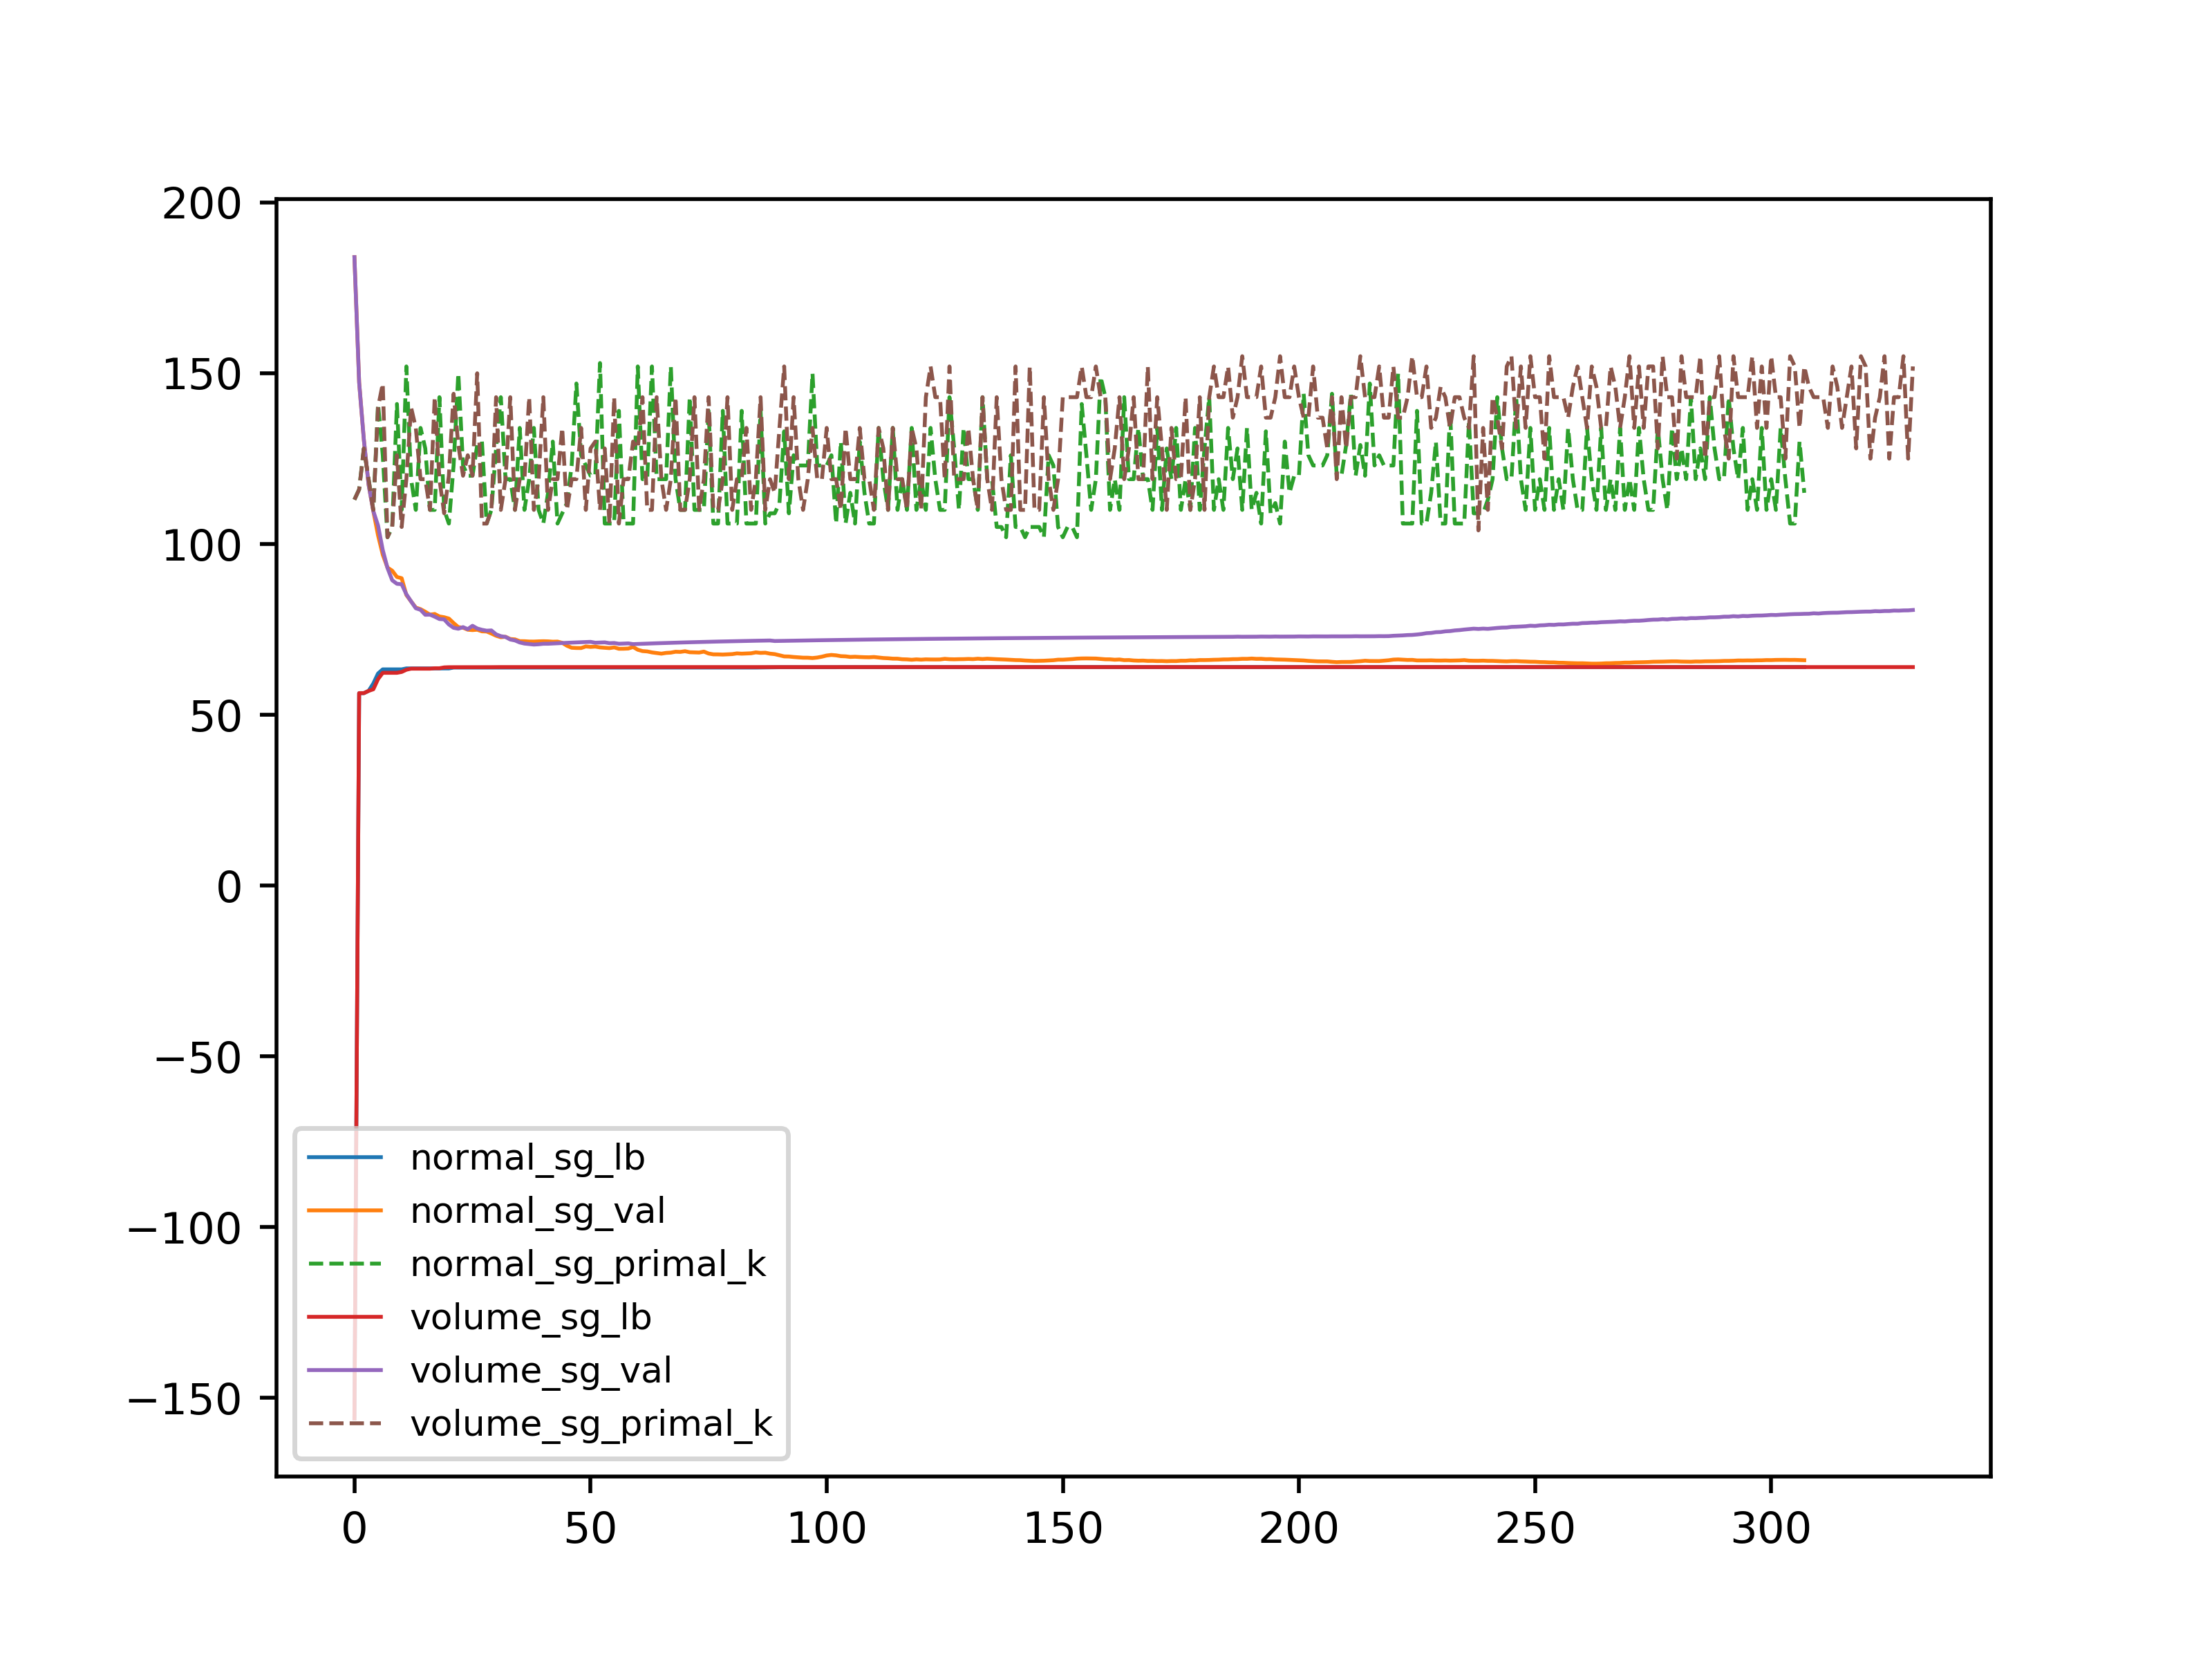
\includegraphics{../imgs/conv_0_15_15.png}\label{fig:divergent_volume}

% finish off
\addcontentsline{toc}{section}{References}

\hypertarget{refs}{}
\bibliography{repair}
\bibliographystyle{informs2014}

\end{document}
